\documentclass{article}
\PassOptionsToPackage{numbers,sort&compress}{natbib}
\usepackage[preprint]{neurips_2026}
\usepackage[T1]{fontenc}
\usepackage[utf8]{inputenc}
\usepackage{microtype}
\usepackage{graphicx}
\usepackage{booktabs}
\usepackage{tabularx}
\usepackage{amsmath,amssymb}
\usepackage{tikz}
\usetikzlibrary{arrows.meta,positioning,calc}
\usepackage{xcolor}
\usepackage{hyperref}
\usepackage{url}
\hypersetup{colorlinks=true,linkcolor=blue!45!black,citecolor=blue!45!black,urlcolor=blue!45!black,
pdftitle={When2Ask: A Benchmark and Jev-Based Clarification Gate for Robotic Tasks},
pdfauthor={Liang Junyi and Yang Haocheng}}
\makeatletter
\renewcommand{\@noticestring}{CS4278/CS5478 Intelligent Robots: Final Project Report. Team 11.}
\makeatother
\setlength{\emergencystretch}{1.5em}
\newcommand{\ask}{\textsc{Ask}}
\newcommand{\cont}{\textsc{Continue}}
\newcommand{\done}{\textsc{Done}}

\title{When2Ask: A Benchmark and Jev-Based\\Clarification Gate for Robotic Tasks}
\author{Liang Junyi \qquad Yang Haocheng\\
Team 11\\
National University of Singapore}

\begin{document}
\raggedbottom
\maketitle

\begin{abstract}
Robotic instructions often omit preferences that determine a correct action.
An agent must decide when to ask for those preferences and when useful work can
continue. We present When2Ask, a benchmark with nine task types that vary
physical layouts, user choices, and information disclosure. We also introduce
Jev-Gate, which separates a binary clarification decision from language-model
question and action generation. Experiments compare conversational models under
the same gate-and-planner workflow, then compare three decision methods with a
shared DeepSeek planner. DeepSeek Flash achieves 100.0\% task success with the
lowest API time and estimated cost among the three evaluated conversational
models. In the shared-planner comparison, Jev-Gate achieves 96.3\% success,
compared with 100.0\% for LLM-Gate and 77.8\% for NoAsk. Jev-Gate uses 30.5\% less
API time and 46.3\% lower estimated API cost than LLM-Gate. These results identify
a concrete trade-off: a separate Jev gate reduces inference overhead while
retaining high task success in the evaluated tasks.
\end{abstract}

\section{Introduction}

Natural-language instructions rarely specify every decision that a robot must
make. A request such as \emph{Put the red cup in my preferred container} names the
object but leaves the destination unresolved. Moving the cup into an arbitrary
container may be physically feasible and still violate the user's intent.
Clarification lets the robot obtain the missing preference before committing
to that choice.

The timing of the question matters. Consider \emph{Open the box, bring my chosen
item, then put the lid back}. The robot can open the box before it knows which
item to retrieve. Asking immediately interrupts work that is already supported
by the instruction. Conversely, postponing the question until after selecting
an item risks an incorrect action. A third situation requires observation:
when a label is hidden behind an obstruction, the robot can uncover and inspect
it. Asking the user to supply that observable fact is unnecessary.

These cases motivate a decision rule based on task progress. The robot should
ask when an unresolved user choice blocks useful required work. It should
continue when a known subgoal or an informative observation remains available.
This rule distinguishes a private preference from a fact that the robot can
measure. It also distinguishes information needed now from information needed
later.

Large language models can interpret instructions and select robot skills
\citep{ahn2022saycan,liang2022code}. However, invoking a conversational model
for every clarification decision adds response time and API cost. The decision
itself has only two outcomes: ask or continue. This suggests separating the
small decision from the richer generation of a question or a robot command.

When2Ask addresses both evaluation and implementation. Its benchmark represents
tasks through public dependencies, physical scenes, and fixed private user
choices. The agent receives observations and interaction history, while an
independent evaluator checks the final state and required task order.
The implementation places a clarification gate before a shared planner.
LLM-Gate uses a conversational model for the gate. Jev-Gate uses a typed
probability from Jev and retains the same downstream planner.

Our contributions are:
\begin{itemize}
  \item A benchmark covering nine manipulation, navigation, and inspection
  task types. It varies layouts, preferences, and disclosure while keeping
  private answers separate from the agent's input.
  \item A Jev-based clarification gate and an empirical comparison of its
  success, API time, and estimated cost against LLM-Gate and a NoAsk baseline.
  A separate cross-model comparison evaluates the conversational models used
  for gating and planning.
\end{itemize}

\paragraph{Project code.}
The implementation and running instructions are available in our
\href{https://github.com/liangjunyi010/when2ask}
{GitHub repository},
on branch \texttt{main}.
Appendix~\ref{app:code} gives the relevant entry points.

\section{Related Work}

\paragraph{Robotic benchmarks.}
LIBERO organizes manipulation tasks around changes in spatial relations,
objects, and goals \citep{liu2023libero}. VIMA-Bench evaluates multimodal task
specification and several levels of generalization \citep{jiang2023vima}.
BEHAVIOR-1K combines activity definitions with diverse objects and scenes
\citep{li2023behavior}. When2Ask focuses on a complementary dimension:
which information is available to an agent, and when obtaining a user answer
is necessary for task progress.

\paragraph{Language models for robot control.}
SayCan combines language-based task relevance with skill affordances to select
actions that a robot can execute \citep{ahn2022saycan}. Code as Policies
generates programs that compose perception and control functions
\citep{liang2022code}. These approaches establish useful ways to connect
language to robot capabilities. When2Ask builds on the same separation between
high-level decisions and executable skills. Its focus is the decision to obtain
missing user information before selecting a skill.

\paragraph{Feedback during execution.}
Inner Monologue incorporates scene descriptions, success feedback, and human
interaction into language-model planning \citep{huang2022inner}. This feedback
allows later decisions to depend on what actually happened. When2Ask similarly
updates the public state after actions and answers. It makes the interaction
decision an explicit component, so the gate can be compared while the planner
and robot interfaces remain fixed.

\paragraph{Knowing when to ask.}
KnowNo uses conformal prediction to align uncertainty in language-model
planning and request help when needed \citep{ren2023knowno}. It provides a
principled treatment of uncertainty and assistance. Our project examines a
different operational question: whether missing user information blocks
useful progress at the current stage of a task. The task dependencies matter
because an unresolved future choice can coexist with a currently executable
subgoal. The benchmark also includes inspection tasks, where an action can
reveal the missing information.

\paragraph{Typed decision models.}
Jev supports a Noul output that represents the probability of a yes/no
proposition \citep{typesafe2026noul}. We use that interface to evaluate whether
clarification is currently required. The returned scalar becomes a gate
decision through a fixed threshold. The downstream language model still
generates the question or action. The contribution is the use and evaluation
of this division of work in a robotic task loop.

\section{Method}

\subsection{Task Representation and Information Access}

Each task consists of an instruction, a dependency graph, a physical layout,
and user-specific choices. The dependency graph is a directed acyclic graph.
Its nodes describe executable subgoals, and its edges specify prerequisites.
For retrieval, opening the box precedes retrieving the selected item, which
precedes replacing the lid.

The agent's public state contains the instruction, task dependencies, current
observation, and action and dialogue history. Observations provide the
task-relevant object and environment information available at that time.
The history records previous actions, their outcomes, questions, and disclosed
answers. A previously supplied preference can therefore be reused without
asking the same question again.

Private user intent remains outside the public state until an appropriate
question requests it. For example, the scene may contain two candidate
containers, while the user's preferred container is stored privately.
The answer module returns only the information requested by the question.
The agent cannot read evaluation labels or the full private intent directly.
The independent evaluator can use the private intent to determine whether the
completed arrangement matches the user's request.

\subsection{Benchmark Construction}

Figure~\ref{fig:tasks} shows the nine task types. They cover manipulation,
navigation, and inspection. The variation is functional: some tasks require an
early preference, some allow useful progress before clarification, and others
require observation rather than a user answer.

\begin{figure}[t]
\centering
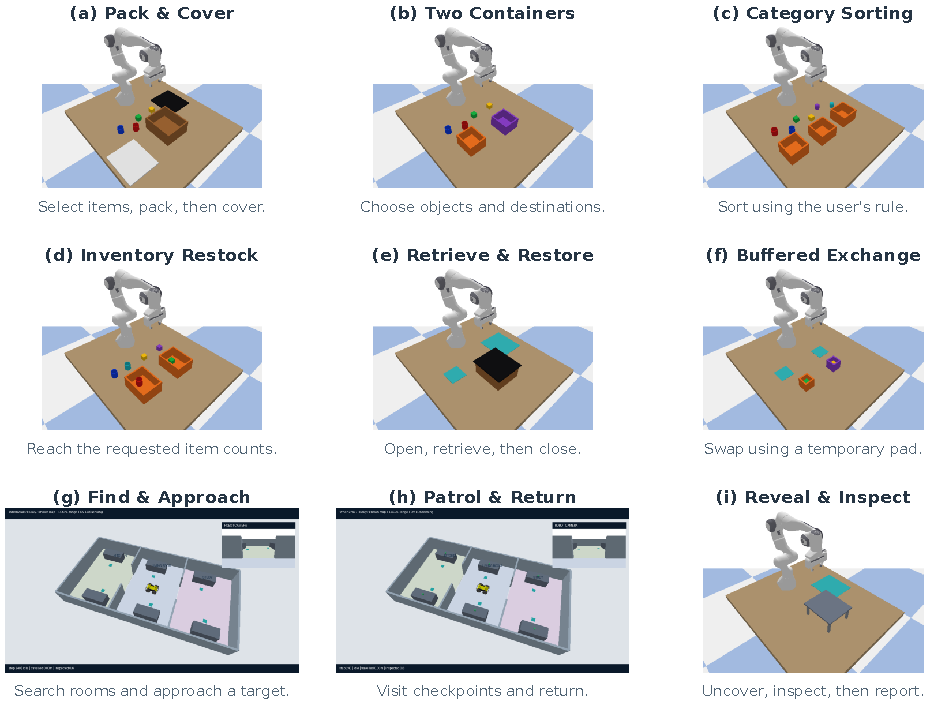
\includegraphics[width=\linewidth]{../graph/figures/task_suite.pdf}
\caption{The nine When2Ask task types. Each scene is paired with a task
instruction and its information-disclosure setting. Six tasks involve
manipulation, two involve navigation, and one involves visual inspection.}
\label{fig:tasks}
\end{figure}

Construction begins with a task template and its public dependency graph.
We instantiate candidate objects and initial poses, assign the user's private
choices, and generate an instruction with a selected amount of information.
Disclosed and undisclosed variants can share a layout, which exposes the
effect of missing information without changing the physical task.
Layout-based grouping keeps related variants together when partitions are
formed.

Each case is checked by executing a scripted solution in PyBullet and evaluating
the final state and task order. This validation confirms that the requested
task can be carried out by the available skills. Model-driven evaluation then
uses the same environment and success conditions, but the agent must choose
its own questions and actions.

The distinction between preferences and observable facts is central to the
benchmark. The robot cannot discover a user's preferred container simply by
looking at the containers. In contrast, moving an obstruction can reveal a
label. The benchmark includes both situations so that asking more questions
alone is not sufficient for correct behavior.

\subsection{Clarification Gate}

The gate receives only the public state and produces \ask{} or \cont{}.
The criterion is whether missing user information blocks useful, supported
task progress now. Physical feasibility is insufficient: the ability to move
either of two objects does not justify guessing which one the user selected.
At the same time, a preference needed for a later subgoal should not prevent
an earlier, fully specified action.

Jev-Gate evaluates this criterion through the Noul interface
\citep{typesafe2026noul,typesafe2026models}. Its decision is
\begin{equation}
g(s_t)=
\begin{cases}
\mathrm{ASK}, & p_{\mathrm{Jev}}(\text{clarification required}\mid s_t)\geq 0.5,\\
\mathrm{CONTINUE}, & \text{otherwise}.
\end{cases}
\label{eq:gate}
\end{equation}
Here, $s_t$ is the current public state. The threshold is fixed at 0.5 for the
reported comparison. Jev selects the branch; it does not choose the object,
write the question, or generate a robot action.

\begin{figure}[t]
\centering
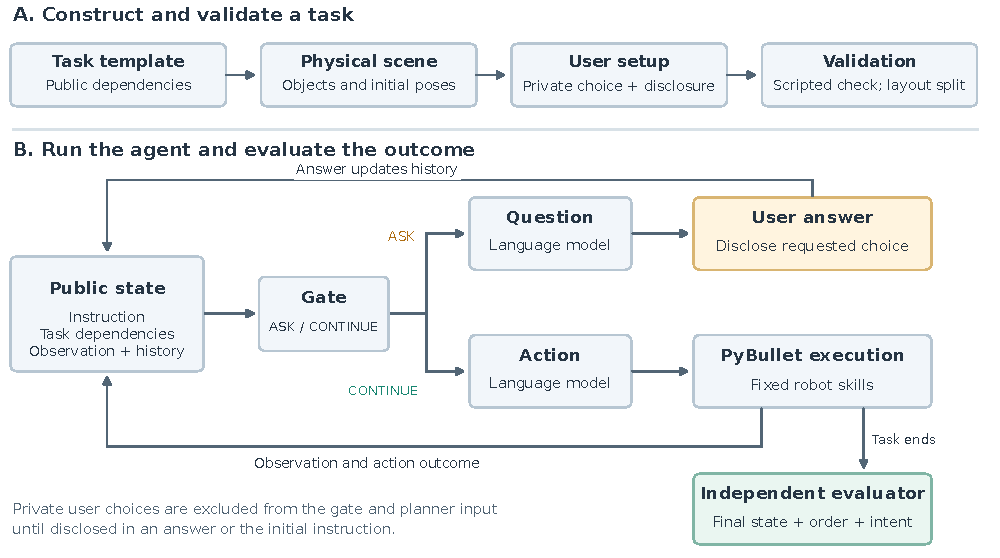
\includegraphics[width=\linewidth]{../graph/figures/benchmark_protocol.pdf}
\caption{Task construction and the execution loop. The gate and planner use
public information. A question reveals the requested user choice, while an
action updates the observation. The evaluator checks the final task outcome
and required order independently of the planner's completion claim.}
\label{fig:loop}
\end{figure}

\subsection{Planning, Answers, and Execution}

Figure~\ref{fig:loop} shows task construction and the decision loop. On \ask{}, the language model
generates a question about the unresolved information. The answer module
discloses the requested value, and the dialogue history is updated.
An answer changes the available information without itself executing a robot
motion. The gate then evaluates the updated state.

On \cont{}, the action planner selects an available robot skill or returns
\done{}. Skills execute in the PyBullet environment \citep{coumans2021pybullet}.
The updated observations and action outcomes become part of the next public
state. Manipulation uses the Panda robot and fixed skills, while navigation
and inspection use their corresponding task interfaces. The language model
operates at the skill level rather than directly controlling joint torques.

The evaluator checks the required final relations and task order independently
of the model's completion claim. A robot can execute a valid movement and
still fail because it selected the wrong object or destination. Conversely,
an intermediate rejected command need not imply final failure if the agent
subsequently completes the task within the execution budget.

\subsection{Compared Methods}

\textbf{LLM-NoAsk} always continues to action planning. It uses DeepSeek to
select actions but cannot request a user answer. This baseline tests what
happens when the planner must act with its available information.

\textbf{LLM-Gate} uses DeepSeek for a separate \ask{}/\cont{} decision.
DeepSeek then generates the corresponding question or action. A decision
cycle therefore includes a gate request followed by a planning request.

\textbf{Jev-Gate} replaces the separate DeepSeek gate with
Equation~\ref{eq:gate}. DeepSeek remains responsible for questions and actions.
The robot skills, answer mechanism, and evaluator remain shared. This
comparison tests the effect of changing the decision component while
retaining the downstream planning workflow.

\section{Experiments}

\subsection{Evaluation Setup and Metrics}

We conduct two comparisons. The cross-model comparison uses the LLM-Gate
workflow throughout. Each selected conversational model serves as both gate
and planner. The shared-planner comparison fixes DeepSeek Flash for question
and action generation, then compares NoAsk, LLM-Gate, and Jev-Gate.

The shared-planner evaluation contains 27 cases across the nine task types,
drawn from 18 base layouts in the development partition. Each method starts
from the same case-specific scene and public information. Cases include
fully disclosed instructions and variants with missing information.
The main comparison therefore contains 27 evaluated episodes per method.
Jev uses threshold 0.5. Task-family execution budgets and success checks are
held constant across methods.

We report four quantities:
\begin{itemize}
  \item \textbf{Task success:} the proportion of episodes that satisfy the
  independent task evaluator, including the requested user choices and order.
  \item \textbf{API time:} accumulated model-request time, averaged per episode.
  It includes the inference needed by the workflow and excludes robot-motion
  time and human-response time.
  \item \textbf{Estimated API cost:} the usage-based dollar estimate per
  episode, using the backend rates associated with the experiment.
  \item \textbf{Unnecessary ASK rate:} the frequency of asking when the
  information already supplied is sufficient. In the shared-planner study,
  this is a task-level measure on 18 fully specified cases.
\end{itemize}

The time and cost measurements describe the whole inference workflow, including
question and action generation. They are not isolated gate microbenchmarks.
For the method comparison, both quantities are normalized to LLM-Gate = 100\%.
The cost values are estimates from API usage, so they are reported separately
from measured request time.

\subsection{Cross-Model Results}

Table~\ref{tab:models} compares the three conversational models.
GPT-5.6 and DeepSeek Flash both achieve 100.0\% task success. GLM 5.2 achieves
93\%. DeepSeek Flash has the lowest average API time, at 8.24 seconds, and the
lowest estimated cost, at \$0.00198 per task.

\begin{table}[t]
\caption{Cross-model evaluation under the LLM-Gate workflow. Each model serves
as both gate and planner. Times and costs are per-task averages.}
\label{tab:models}
\centering
\small
\begin{tabular*}{\linewidth}{@{\extracolsep{\fill}}lrrrr@{}}
\toprule
API model & Task success & API time & Est.\ API cost & Unnecessary ASK \\
\midrule
GPT-5.6 & 100.0\% & 12.52 s & \$0.02541 & 0.0\% \\
DeepSeek Flash & 100.0\% & 8.24 s & \$0.00198 & 0.0\% \\
GLM 5.2 & 93\% & 10.12 s & \$0.00302 & 4\% \\
\bottomrule
\end{tabular*}
\end{table}

These results support the choice of DeepSeek Flash as the shared planner.
It matches the highest observed success rate while requiring less API time
and lower estimated cost than the other evaluated models. The comparison
also separates planner selection from gate design: subsequent differences
between LLM-Gate and Jev-Gate are measured with the same DeepSeek planner,
rather than with different conversational models in their planning stages.

\subsection{Shared-Planner Results}

Figure~\ref{fig:results} reports the three-method comparison.
NoAsk succeeds on 77.8\% of tasks. LLM-Gate reaches 100.0\%, while Jev-Gate
reaches 96.3\%. Both methods with a clarification gate achieve higher observed
success than the baseline that always proceeds.

\begin{figure}[t]
\centering
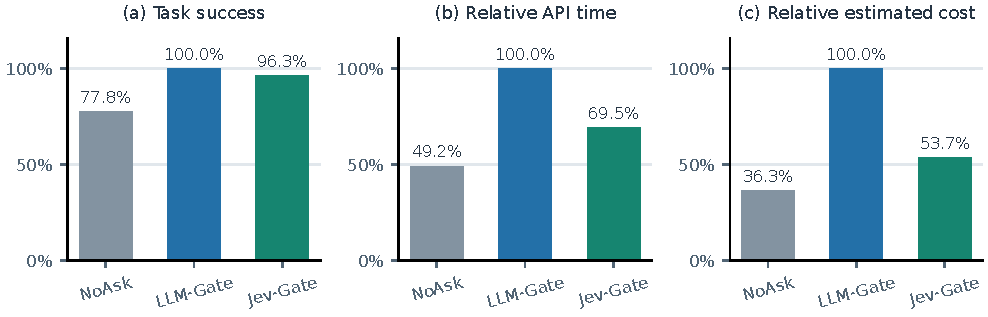
\includegraphics[width=\linewidth]{../graph/figures/aggregate_comparison.pdf}
\caption{Shared-planner comparison on the same 27 nine-task development
cases. API time and estimated cost are relative to LLM-Gate = 100\%.
Lower values are better for time and cost; higher values are better for
success.}
\label{fig:results}
\end{figure}

Jev-Gate uses 69.5\% of LLM-Gate's API time and 53.7\% of its estimated cost.
Equivalently, it reduces API time by 30.5\% and estimated cost by 46.3\%.
The associated success difference is 3.7 percentage points. This is the main
result of the method comparison: the separate Jev gate retains high success
while reducing the inference overhead of a separate conversational gate.

NoAsk uses the least API time and estimated cost, at 49.2\% and 36.3\% of the
LLM-Gate baseline. This lower inference overhead accompanies a lower
success rate. Jev-Gate occupies a different operating point: it
retains the ability to ask, gives substantially higher observed success than
NoAsk, and uses less inference time and estimated cost than LLM-Gate.

Neither gate method produces an unnecessary ASK in the fully specified control
cases. The observed rate is therefore 0\% for both. NoAsk has no clarification
gate, so this metric is not applicable to it. Reporting NoAsk as having a
perfect gate score would obscure the fact that it is prohibited from asking.

Together, the success and overhead results answer the method research
question. Replacing the LLM gate with Jev is an effective option when lower
inference overhead is important and the measured success trade-off is
acceptable. LLM-Gate remains the highest-success method in this comparison.
The choice depends on the operating requirement rather than on one metric
alone. Appendix~\ref{app:breakdown} provides the per-task success counts
and a joint view of success and inference overhead.

\subsection{Clarification Timing and Interaction}

Figure~\ref{fig:examples} shows two recorded Jev-Gate episodes from the
shared-planner study. In Retrieve \& Restore, the robot opens the box before
asking which item to retrieve. After receiving the answer, it delivers the
cup and replaces the lid. In Reveal \& Inspect, it moves the screen, inspects
the label, and reports the observed code without asking. Both episodes pass
the task evaluator. These examples show how the same gate handles a private
preference and an observable fact.

\begin{figure}[t]
\centering
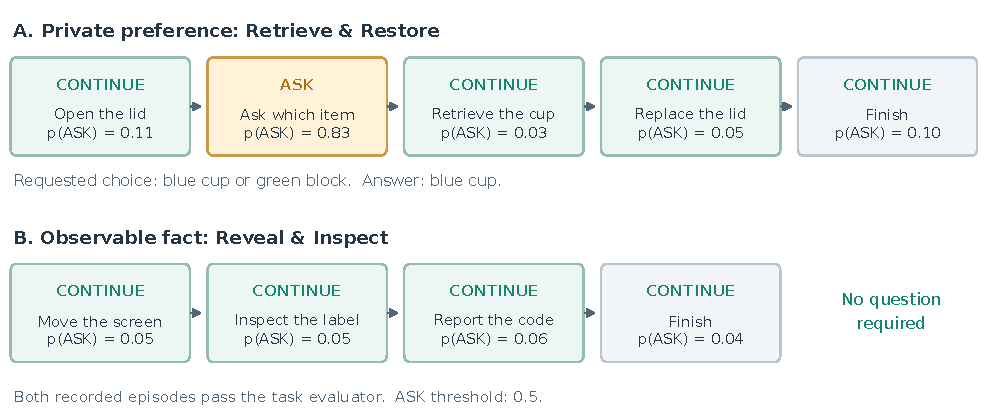
\includegraphics[width=\linewidth]{../graph/figures/clarification_examples.pdf}
\caption{Recorded decision sequences for two Jev-Gate episodes. The numbers
are the returned ASK probabilities, with a threshold of 0.5. Action and
dialogue descriptions are shortened for readability. The first task asks
only after useful initial progress; the second obtains the information
through inspection.}
\label{fig:examples}
\end{figure}

The command-center demonstration also runs four tasks in independent
PyBullet worlds. When one agent asks, its task waits for the answer while the
others can continue. The answer updates that agent's history and execution
resumes. All four tasks complete in the recorded demonstration, with success
checked by the task evaluators.

\subsection{Discussion and Scope}

The evaluator measures complete task outcomes because a correct gate decision
does not guarantee correct planning or execution. Gate decisions also affect
the number and timing of downstream requests. The reported time and cost
therefore reflect the complete interaction trajectories, including their
token usage and the service rates used in the experiment.

The present evaluation covers predefined task structures and fixed robot
skills in PyBullet. The cases vary layout, preference, and disclosure within
those structures. Extending the benchmark to new task structures and deploying
the decision loop on physical robot hardware are useful next steps.
Broader testing can also examine more complex preferences and longer
interaction histories. These extensions build on the demonstrated
success--overhead trade-off.

\section{Conclusion}

When2Ask provides a benchmark for deciding when a robotic agent should ask for
missing information and when it should continue useful work. Its nine task
types combine public dependencies, controlled user choices, and independent
task evaluation.

The experiments lead to two conclusions. DeepSeek Flash achieves the best
observed combination of success, API time, and estimated cost among the three
conversational models evaluated under the same workflow. With that planner
fixed, Jev-Gate achieves 96.3\% task success while reducing API time by 30.5\%
and estimated cost by 46.3\% relative to LLM-Gate. LLM-Gate achieves 100.0\%
success, so the saving comes with a measured success trade-off.

The practical contribution is an explicit clarification decision that can be
implemented by a separate typed model while a conversational model retains
question and action generation. This design offers a useful way to reduce
inference overhead without removing the ability to obtain necessary user
information.

\clearpage
\bibliographystyle{unsrtnat}
\bibliography{references_illustrated}

\clearpage
\appendix
\section{Code and Running Instructions}
\label{app:code}

The \href{https://github.com/liangjunyi010/when2ask}{project repository}
includes the code, saved results, and setup instructions. The commands below
clone the main branch and install the
project in its Python 3.11 environment.

\begin{verbatim}
git clone https://github.com/liangjunyi010/when2ask.git
cd when2ask
bash script/setup_env.sh
.venv/bin/python script/benchmark.py doctor
\end{verbatim}

The saved evaluation can be inspected without making model requests:
\begin{verbatim}
.venv/bin/python script/benchmark.py report
.venv/bin/python script/benchmark.py audit
\end{verbatim}

\noindent Useful entry points are:
\begin{itemize}
  \item \texttt{result/EXPERIMENT.md}: evaluation protocol,
  metric definitions, and recorded outcomes.
  \item \texttt{script/benchmark.py}: physical validation, execution,
  reporting, and audit commands.
  \item \texttt{result/nine\_task\_metrics\_dev\_v1/}: saved episode evidence
  and the generated result tables.
  \item \texttt{src/when2ask/}: the gate, planner, environment, task definitions,
  and independent evaluators.
\end{itemize}

Live evaluation requires locally configured API credentials. The run command
uses an explicit \texttt{--live} option. Saved study artifacts are preserved
by the runner, so a new evaluation should use a separately configured run
rather than overwrite an existing study.


\clearpage
\section{Task Breakdown and Efficiency}
\label{app:breakdown}

Figure~\ref{fig:task_counts} breaks down the same 27 evaluation cases used in
the main comparison. Each task type has three cases. The counts sum to 21
successes for NoAsk, 27 for LLM-Gate, and 26 for Jev-Gate. Jev-Gate's single
unsuccessful case is in Inventory Restock. These are descriptive counts for
the evaluated cases.

\begin{figure}[h!]
\centering
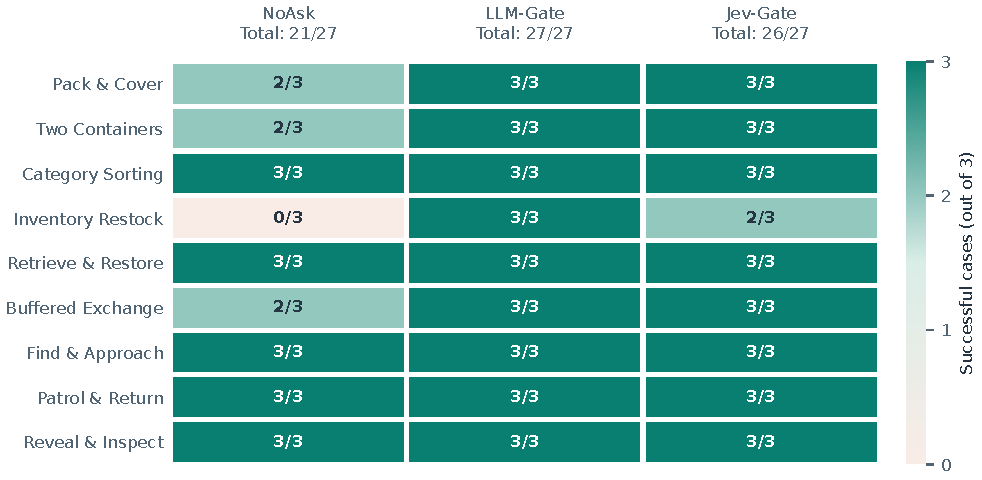
\includegraphics[width=0.92\linewidth]{../graph/figures/task_success_heatmap.pdf}
\caption{Successful cases by task and method. Every cell has the same
denominator of three cases. The totals agree with the aggregate success
rates in Figure~\ref{fig:results}.}
\label{fig:task_counts}
\end{figure}

\begin{figure}[h!]
\centering
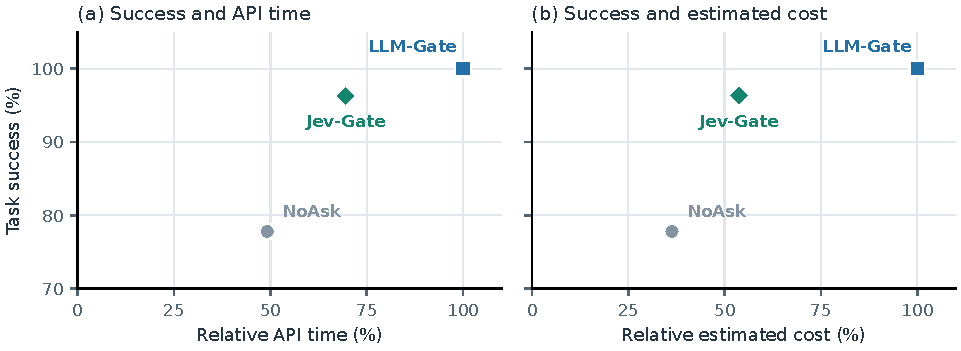
\includegraphics[width=\linewidth]{../graph/figures/efficiency_tradeoff.pdf}
\caption{Success and inference overhead for the three methods. Each point
uses the same aggregate values as Figure~\ref{fig:results}. API time and
estimated cost are relative to LLM-Gate = 100\%. Higher success and lower
inference overhead are preferable.}
\label{fig:tradeoff}
\end{figure}

\end{document}
